\section{Wiring a Watts-Strogatz Graph} \label{sec:proof4}

Consider a set of computational nodes arranged in an $r$-dimensional mesh.
In each dimension, physical interconnects run between immediately adjacent pairs of nodes.
Represent this physical hardware with a graph $N$.
Vertices of $N$, $V(N)$, represent computational nodes.
Edges of $N$, $E(N)$, represent physical interconnects between nodes.

Let $d(a,b)$ represent the typical number of physical interconnects traversed on a shortest path between a pair of arbitrary nodes $a, b \in V(N)$.
This is conceptually equivalent to Manhattan distance.

In the case of a one-dimensional sequence of nodes, for a pair of arbitrary nodes $a,b \in V(N)$,
\begin{align*}
\bar{d}(a,b) \propto |V(N)|.
\end{align*}

Consider next the case of a higher-dimensional grid topology, like a two-dimensional grid or a three-dimensional mesh.
Because $d$ is a Manhattan metric, the number of physical interconnects requiring traversal in each dimension on a shortest-path between two nodes is completely independent.

Arranging the set of nodes $N$ in a $r$-dimensional cube, cube width in each dimensions scales proportionally to the $r$-th root of $|V(N)|$.

So, for a pair of arbitrary nodes $a,b \in V(N)$,
\begin{align} \label{eqn:mesh_prop}
\bar{d}(a, b) \propto |V(N)|^{\frac{1}{r}} \times r
\end{align}

We proceed to construct a small world directed graph $G$ using the set of nodes $N$ as vertices.
In formal terms, a bijective relationship $f: V(N) \rightarrow V(G)$ unites these two sets.
The inverse mapping, $f^{-1}: V(G) \rightarrow V(N)$, is also bijective.

\begin{figure}[t]
\begin{center}
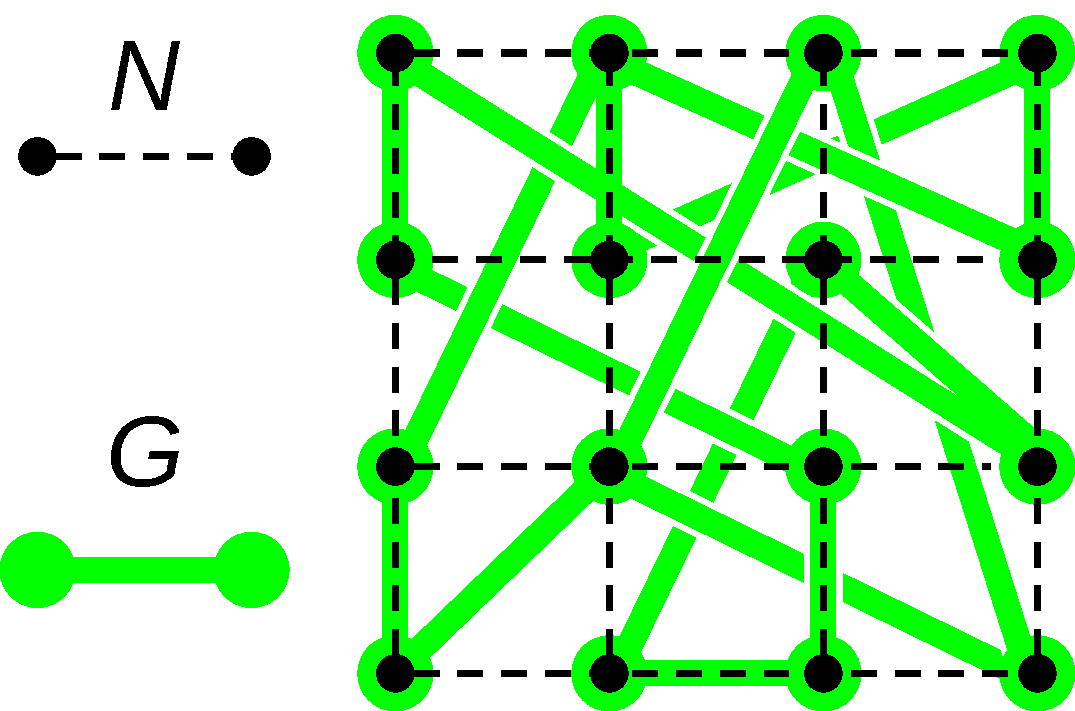
\includegraphics[width=\linewidth]{nandg}
\caption{
TODO
}
\label{fig:nandg}
\end{center}
\end{figure}


Edges in the graph $G$ do not represent a physical interconnect.
Instead, edges $\{\hat{a}, \hat{b}\} \in E(G)$ represent a close-coordination relationship where node $\hat{a}$ frequently interacts with (i.e., dispatches messages to) the destination node $\hat{b}$.
Figure \ref{fig:nandg} illustrates the relationship between $N$ and $G$.

Let $\hat{d}(\hat{a},\hat{b})$ denote distance between vertices $\hat{a}$ and $\hat{b}$ with respect to the graph $G$.
That is, the number of graph edges traversed on a shortest-path route between $\hat{a}$ and $\hat{b}$ over $G$.
In a small-world network, typical graph distance scales proportionally with the logarithm of network size \citeinappendix{watts1998collective}.
In our case, for arbitrary $\hat{a},\hat{b} \in V(G)$,
\begin{align} \label{eqn:smallworld_prop}
\bar{\hat{d}}(\hat{a},\hat{b}) \propto \log(|V(G)|).
\end{align}

Suppose we have a small-world graph $G$ constructed over a mesh $N$ (as in Figure \ref{fig:nandg}) using the Watts–Strogatz algorithm.
In this procedure, vertices in $V(G)$ corresponding to neighboring computational nodes in $V(N)$ are wired together to form a lattice with mean degree $k$.
Then, for every vertex $v \in V(G)$, each edge $\{x, y\} \in E(G)$ containing $v$ is reconfigured with probability $0 < \beta < 1$ to connect $v$ to a randomly-chosen node $w \in V(G)$.

Before reconfiguration, the total wiring cost of $G$ with respect to hops over $N$ was proportional to $|V(G)|$.

Recall that, with mesh dimensionality $r$ we know that for a pair of arbitrary nodes $a,b \in V(N)$,
\begin{align*}
\bar{d}(a, b) \propto |V(N)|^{\frac{1}{r}} \times r.
\end{align*}

So, after rewiring, the total wiring cost $w$ of $G$ with respect to hops over $N$ can be calculated as
\begin{align*}
  \beta |V(G)| \times |V(N)|^{\frac{1}{r}} \times r + (1 - \beta) |V(G)|.
  %\\
  % \beta |V(N)| \times |V(N)|^{\frac{1}{r}} \times r + (1 - \beta) |V(N)|.
  % \beta |V(N)|^{\frac{r+1}{r}} \times r + (1 - \beta) |V(N)|.
\end{align*}

So, $w \in \Omega \Big( |V(N)|^{\frac{r+1}{r}} \times r \Big).$

In this graph, the number of edges is proportional to the graph size $n$.

With bounded mean degree, we have $|E(G)| \propto |V(G)|$ so we can establish the following lower bound on mean wiring cost per edge of $G$ with respect to hops over $N$,
\begin{align*}
\Omega \Big( |V(G)|^{\frac{1}{r}}| \times r \Big).
\end{align*}

Note that, with the introduction of log-time hierarchical hardware interconnects into $N$ the mean wiring cost per edge of $G$ with respect to hops over $N$ is bounded in the worst case by $\Omega \Big( \log |V(G)| \Big)$.
